\pdfminorversion=4
\documentclass[aspectratio=169]{beamer}

\mode<presentation>
{
  \usetheme{default}
  \usecolortheme{default}
  \usefonttheme{default}
  \setbeamertemplate{navigation symbols}{}
  \setbeamertemplate{caption}[numbered]
  \setbeamertemplate{footline}[frame number]  % or "page number"
  \setbeamercolor{frametitle}{fg=white}
  \setbeamercolor{footline}{fg=black}
} 

\usepackage[english]{babel}
\usepackage[utf8x]{inputenc}
\usepackage{tikz}
\usepackage{courier}
\usepackage{array}
\usepackage{bold-extra}
\usepackage{minted}
\usepackage[thicklines]{cancel}
\usepackage{fancyvrb}

\xdefinecolor{dianablue}{rgb}{0.18,0.24,0.31}
\xdefinecolor{darkblue}{rgb}{0.1,0.1,0.7}
\xdefinecolor{darkgreen}{rgb}{0,0.5,0}
\xdefinecolor{darkgrey}{rgb}{0.35,0.35,0.35}
\xdefinecolor{darkorange}{rgb}{0.8,0.5,0}
\xdefinecolor{darkred}{rgb}{0.7,0,0}
\definecolor{darkgreen}{rgb}{0,0.6,0}
\definecolor{mauve}{rgb}{0.58,0,0.82}

\title[2019-04-17-irishep-awkwardnumba]{Awkward Array: Numba}
\author{Jim Pivarski}
\institute{Princeton University -- IRIS-HEP}
\date{April 17, 2019}

\usetikzlibrary{shapes.callouts}

\begin{document}

\logo{\pgfputat{\pgfxy(0.11, 7.4)}{\pgfbox[right,base]{\tikz{\filldraw[fill=dianablue, draw=none] (0 cm, 0 cm) rectangle (50 cm, 1 cm);}\mbox{\hspace{-8 cm}
\includegraphics[height=1 cm]{princeton-logo-long.png}\hspace{0.1 cm}\raisebox{0.1 cm}{
\includegraphics[height=0.8 cm]{iris-hep-logo-long.png}}\hspace{0.1 cm}}}}}

\begin{frame}
  \titlepage
\end{frame}

\logo{\pgfputat{\pgfxy(0.11, 7.4)}{\pgfbox[right,base]{\tikz{\filldraw[fill=dianablue, draw=none] (0 cm, 0 cm) rectangle (50 cm, 1 cm);}\mbox{\hspace{-8 cm}
\includegraphics[height=1 cm]{princeton-logo.png}\hspace{0.1 cm}\raisebox{0.1 cm}{
\includegraphics[height=0.8 cm]{iris-hep-logo.png}}\hspace{0.1 cm}}}}}

% Uncomment these lines for an automatically generated outline.
%\begin{frame}{Outline}
%  \tableofcontents
%\end{frame}

% START START START START START START START START START START START START START

\begin{frame}{Knowing your audience}
\vspace{0.5 cm}
{\large I presented an ``Accelerating Python'' tutorial to non-particle physics scientists:}

\small
\begin{itemize}\setlength{\itemsep}{-0.1 cm}
\item 8 Computer Science/Software Engineering/Electrical Engineering
\item 7 Physics/Astronomy/Energy Science/Atmospheric \& Ocean Science
\item 5 Finance/Business/Political Science
\item 2 Neuroscience
\item 2 Civil Engineering
\end{itemize}

\large
\vspace{0.5 cm}
\uncover<2->{I started by showing how for-loopy code must be fundamentally rewritten to take advantage of Numpy and why it might be worth the effort.}

\vspace{0.5 cm}
\uncover<3->{\textcolor{darkblue}{Surprise!} They were more comfortable with the \mbox{vectorized form (Numpy/Pandas)---\hspace{-0.5 cm}} for loops were {\it less familiar}.}
\end{frame}

\begin{frame}[fragile]{Knowing your audience}
\large
\vspace{0.5 cm}
Regardless of which side of the divide you start from, \textcolor{darkblue}{event-at-a-time} and \textcolor{darkblue}{operation-at-a-time} approaches are rather different and have different advantages.

\vspace{0.25 cm}
\begin{columns}[t]
\column{0.47\linewidth}
\textcolor{darkblue}{\underline{event-at-a-time}}

{\small
\begin{minted}[stripnl=false]{python}
for event in everything:
    a = step1(event)
    b = step2(a)
    write_one(b)
\end{minted}
}

\begin{itemize}
\item<2-> Good for debugging: insert breakpoints, watch variables to understand a single event.
\item<3-> Detail can obscure big picture.
\end{itemize}

\column{0.46\linewidth}
\textcolor{darkblue}{\underline{operation-at-a-time}}

{\small
\begin{minted}[stripnl=false]{python}
a = step1(everything)
b = step2(a)
write_all(b)

\end{minted}
}

\begin{itemize}
\item<4-> Composition of functions can read like natural language.
\item<5-> Indexes can be hard to align: ``error driven development!''
\end{itemize}

\end{columns}
\end{frame}

\begin{frame}{}
\vspace{1 cm}
\large
\begin{center}
Most talks on awkward-array (including this meeting) are about \\ the value of introducing \textcolor{darkblue}{operation-at-a-time} into particle physics.

\vspace{1 cm}
This talk will be about getting \textcolor{darkblue}{event-at-a-time} in Python without a speed penalty.

\vspace{0.15 cm}
\uncover<2->{\textcolor{darkorange}{\bf Programming strategy should be a {\it separate question} from performance.}}
\end{center}
\end{frame}

\begin{frame}{}
\begin{columns}
\column{1.2\linewidth}
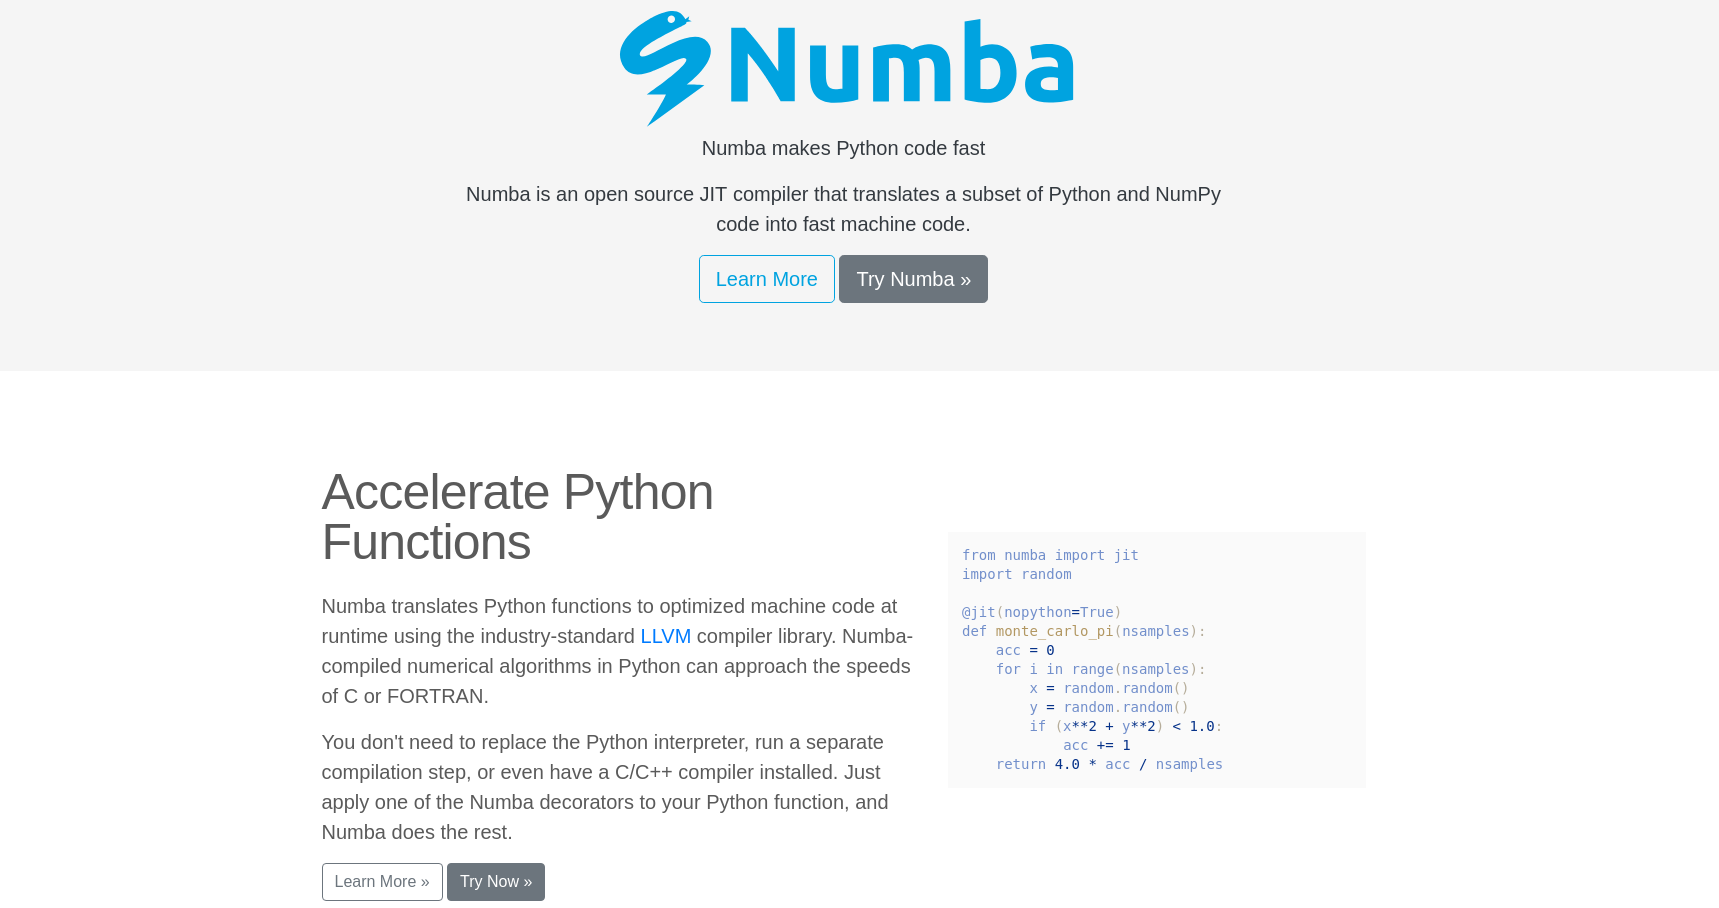
\includegraphics[width=\linewidth]{numba-website.png}
\end{columns}
\end{frame}

\begin{frame}{I've been using Numba for more than 2 years\ldots}
\vspace{0.5 cm}
{\large \ldots and it always wins in my ease-of-use judgements and performance tests.}

\begin{center}
\begin{tabular}{l c r c}
{\bf Method}               & {\bf Configuration} & {\bf Speedup} & {\bf Cores} \\\hline
Pure Python                & for-loopy           &     $1\times$ & 1 \\
Numba                      & for-loopy           &    $50\times$ & 1 \\
Numba-parallel             & for-loopy           &   $165\times$ & all (12) \\
Numpy                      & columnar            &    $15\times$ & 1 \\
CuPy                       & columnar            &    $77\times$ & GPU \\
Dask                       & columnar            &    $26\times$ & all (12) \\
Numba-CUDA                 & CUDA details        &   $800\times$ & GPU \\
pybind11 {\tt -O3}         & for-loopy C++       &    $34\times$ & 1 \\
pybind11 {\tt -ffast-math} & for-loopy C++       &    $90\times$ & 1 \\
Cython                     & dual language       &   $3.7\times$ & 1 \\
\end{tabular}
\end{center}

\textcolor{gray}{(Sorted by my ease-of-use judgement. Iterative fractal example in my tutorials.)}
\end{frame}

\begin{frame}{}

\end{frame}

\end{document}
